\documentclass{standalone}
\usepackage{tikz}

\begin{document}

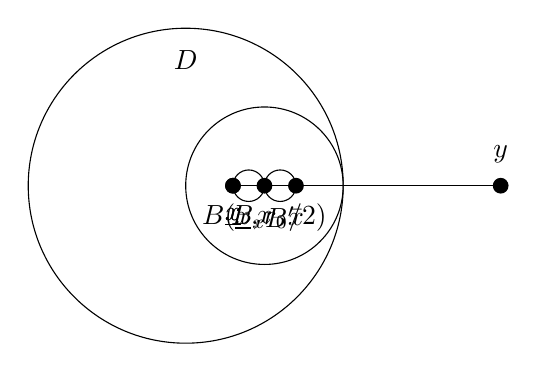
\begin{tikzpicture}[scale=2]
    % Draw the large circle representing D
    \draw (0,0) circle (1);
    
    % Label the large circle as D
    \node at (0,0.8) {$D$};
    
    % Draw the smaller circle representing B(\underline{x}, r_0/2)
    \draw (0.5,0) circle (0.5);
    
    % Label the smaller circle
    \node at (0.5,-0.2) {$B(\underline{x}, r_0/2)$};
    
    % Draw the point y
    \fill (2,0) circle (0.05);
    \node at (2,0.2) {$y$};
    
    % Draw the line from y to the center of the smaller circle
    \draw (2,0) -- (0.5,0);
    
    % Draw the points x and x'
    \fill (0.3,0) circle (0.05);
    \node at (0.3,-0.2) {$\underline{x}$};
    \fill (0.7,0) circle (0.05);
    \node at (0.7,-0.2) {$\bar{x}$};
    
    % Draw the circles B_x and B'
    \draw (0.4,0) circle (0.1);
    \node at (0.4,-0.2) {$B_x$};
    \draw (0.6,0) circle (0.1);
    \node at (0.6,-0.2) {$B'$};
    
    % Draw the point x
    \fill (0.5,0) circle (0.05);
    \node at (0.5,-0.2) {$x$};
    
    % Draw the line segment connecting x and x'
    \draw (0.3,0) -- (0.7,0);
    
    % Draw the point \underline{x}
    \fill (0.3,0) circle (0.05);
    \node at (0.3,-0.2) {$\underline{x}$};
    
\end{tikzpicture}

\end{document}